\documentclass[10pt,a4paper]{article}
	\usepackage[latin1]{inputenc}
	\usepackage{amsmath}
	\usepackage{amsfonts}
	\usepackage{amssymb}
	\usepackage{graphicx}
\begin{document}
\begin{titlepage}

\newcommand{\HRule}{\rule{\linewidth}{0.5mm}} % Defines a new command for the horizontal lines, change thickness here

\center % Center everything on the page
 
%----------------------------------------------------------------------------------------
%	HEADING SECTIONS
%----------------------------------------------------------------------------------------

\textsc{\LARGE Mälardalen university Sweden}\\[1.5cm] % Name of your university/college
\textsc{\Large Robotics project course }\\[0.5cm] % Major heading such as course name
\textsc{\large CDT508/DVA410 30hp}\\[0.5cm] % Minor heading such as course title

%----------------------------------------------------------------------------------------
%	TITLE SECTION
%----------------------------------------------------------------------------------------

\HRule \\[0.4cm]
{ \huge \bfseries Test plan for Naiad}\\[0.4cm] % Title of your document
\HRule \\[1.5cm]
 
%----------------------------------------------------------------------------------------
%	AUTHOR SECTION
%----------------------------------------------------------------------------------------

\large
\emph{Author:}\\
Weronica Kovala \textit{et al.} \\ wrg10002@student.mdh.se % Your name
\vspace{0.3cm}
\\

\emph{Supervisor:} \\
Mikael Ekström \\
mikael.ekstrom@mdh.se
\vspace{1cm}

% If you don't want a supervisor, uncomment the two lines below and remove the section above
%\Large \emph{Author:}\\
%John \textsc{Smith}\\[3cm] % Your name

%----------------------------------------------------------------------------------------
%	DATE SECTION
%----------------------------------------------------------------------------------------

{\large \today}\\[0.5cm]
Not for distribution % Date, change the \today to a set date if you want to be precise

%----------------------------------------------------------------------------------------
%	LOGO SECTION
%----------------------------------------------------------------------------------------

%\includegraphics{Logo}\\[1cm] % Include a department/university logo - this will require the graphicx package
 
%----------------------------------------------------------------------------------------

\vfill % Fill the rest of the page with whitespace

\end{titlepage}
\section{Introduction}
The goal for the tests described in this test plan is to get the Naiad robot ready for competing in robosub 2015 in San Diego, USA. Therefore tests of the mechanics, electronics and software will be conducted. 
\section{Testing}
The testing will test a number of different things involving the whole system. 
\subsection{What will be tested}
The hull, other mechanics, the software and all electronics will be tested at different stages. 
\subsection{What will not be tested}
Since only one copy of the Naiad will be made in this phase of the project, it is not possible to test the robot to robot communication.


\section*{Mechanic tests}
In this section different tests of the mechanics will be described.
\section{Unit test}
Following is a series of tests that should be performed on the mechanical parts of the system. 

\subsection{Testing the o-ring}
\label{oring}
\subsubsection*{Purpouse of the test case}
The purpouse of this test is to make sure that there are no dents in the o-ring, which would make it unsafe to use under water. 
\subsubsection*{Description}
For this test a person will feel through the o-ring to make sure that there are no dents in it. 
\subsubsection*{Resources}
O-ring, petroleum jelly
\subsubsection*{Preconditions}
The preconditions are that the o-ring is dry and grease free. 
\subsubsection*{Post conditions}
After preforming this test the o-ring should be greased and for a pass it should have no dents. Any dents will count as a fail in this test. 
\subsubsection*{Flow of events}
For this test the person performing the test should have some petroleum jelly on their fingers and gently feel every piece of the o-ring to make sure that there are no dents in it. Make sure that the entire o-ring is properly greased. 
\begin{tabular}{| l | c |}
\hline
Check point & Measured \\ \hline
Check for dents &  \\ \hline
\end{tabular}
\subsubsection*{Inclusion/Exclusion points}
The test will count as a pass if the o-ring is free of dents and can be completely greased. All other cases will count as a fail. 
\subsubsection*{Special requirements}
There are no special requirements for this test. 

\subsection{Closing of the hull}
\label{Hulltest}
\subsubsection*{Purpouse of the test case}
This test is supposed to make sure that the hull is water tight when closed. 
\subsubsection*{Description}
The test is done to make sure that the lid is closed properly to make sure there is no leakage when the AUV is put into water. 
\subsubsection*{Resources}
Required resources for this test is the hull of Naiad, some paper, petroleum jelly, a long rope, and weights (for example in a weight belt for diving). 
\subsubsection*{Preconditions}
There are no preconditions for this test. 
\subsubsection*{Post conditions}
After preforming this test the lid of the hull should be closed and the hull should be waterproof. 
\subsubsection*{Flow of events}
Firstly, the hull should be fitted with either the electronics, for an actual run with the robot, or with paper for testing the waterproofness of the hull. 

Then the o-ring should be tested, this is done through feeling the o-ring all the way around using petroleum jelly to grease it thoroughly, for a closer description of this see \ref{oring}. Then it should be placed in the o-ring slot which before hand should be greased as well. Then the lid can be placed and closed to ensure waterproofing. When placing the lid, make sure that no cables are being pinched between the hull and the lid. Also make sure to place the lid from straight above so that the o-ring stays in place. 

\begin{tabular}{| l | c |}
\hline
Check point & Measured \\ \hline
Test of o-ring &  \\ \hline
Placement of o-ring &  \\ \hline
Placement of lid &  \\ \hline
Cable check & \\ \hline
\end{tabular} 
\subsubsection*{Inclusion/Exclusion points}
This test will not test which pressure the hull can sustain, it will just test that there will not be any immediate leakage. 
\subsubsection*{Special requirements}
There are no special requirements for this test. 

\section*{System test}
These tests can be looked at as sort of a flow chart of what to do if something is not working as it is supposed to. 
\section{System test}
Below is a list of a number of tests that should be performed when the system is not working properly in some way.
\subsection{List of tests to be written}
\begin{enumerate}

\item A sensor is giving out a faulty value PÅBÖRJAD, EJ KLAR! 

\end{enumerate}

\subsection{Name of test here}
\subsubsection*{Purpouse of the test case}
\subsubsection*{Description}
\subsubsection*{Resources}
\subsubsection*{Preconditions}
\subsubsection*{Post conditions}
\subsubsection*{Flow of events}
\subsubsection*{Inclusion/Exclusion points}
\subsubsection*{Special requirements}

\subsection{The vision system is not working properly}
\subsubsection*{Purpouse of the test case}
The purpouse of this test case is to find the problem when the GIMME-2 board is not working properly. 
\subsubsection*{Description}
There are a number of different problems that can occur when using the GIMME-2 in Naiad. This test is designed so that finding the problem should be easier.
\subsubsection*{Resources}
Electronics of Naiad including at least one GIMME-2 board with lenses on the camera sensors and a multi-meter. 
\subsubsection*{Preconditions}
Before starting this test the electronics should be powered up and the system should try taking and analysing pictures from the GIMME-2, however for this test to be relevant there has to be a problem somewhere in this process. 
\subsubsection*{Post conditions}
The goal for this test is that the GIMME-2-system should be working properly. 
\subsubsection*{Flow of events}
First thing to check is that the GIMME-2 is powered correctly. Check this using a multi-meter, there should be 12 V where the GIMME-2 is powered see fig. \ref{GimmePower}. 
\begin{figure}[!ht]
	\begin{center}
		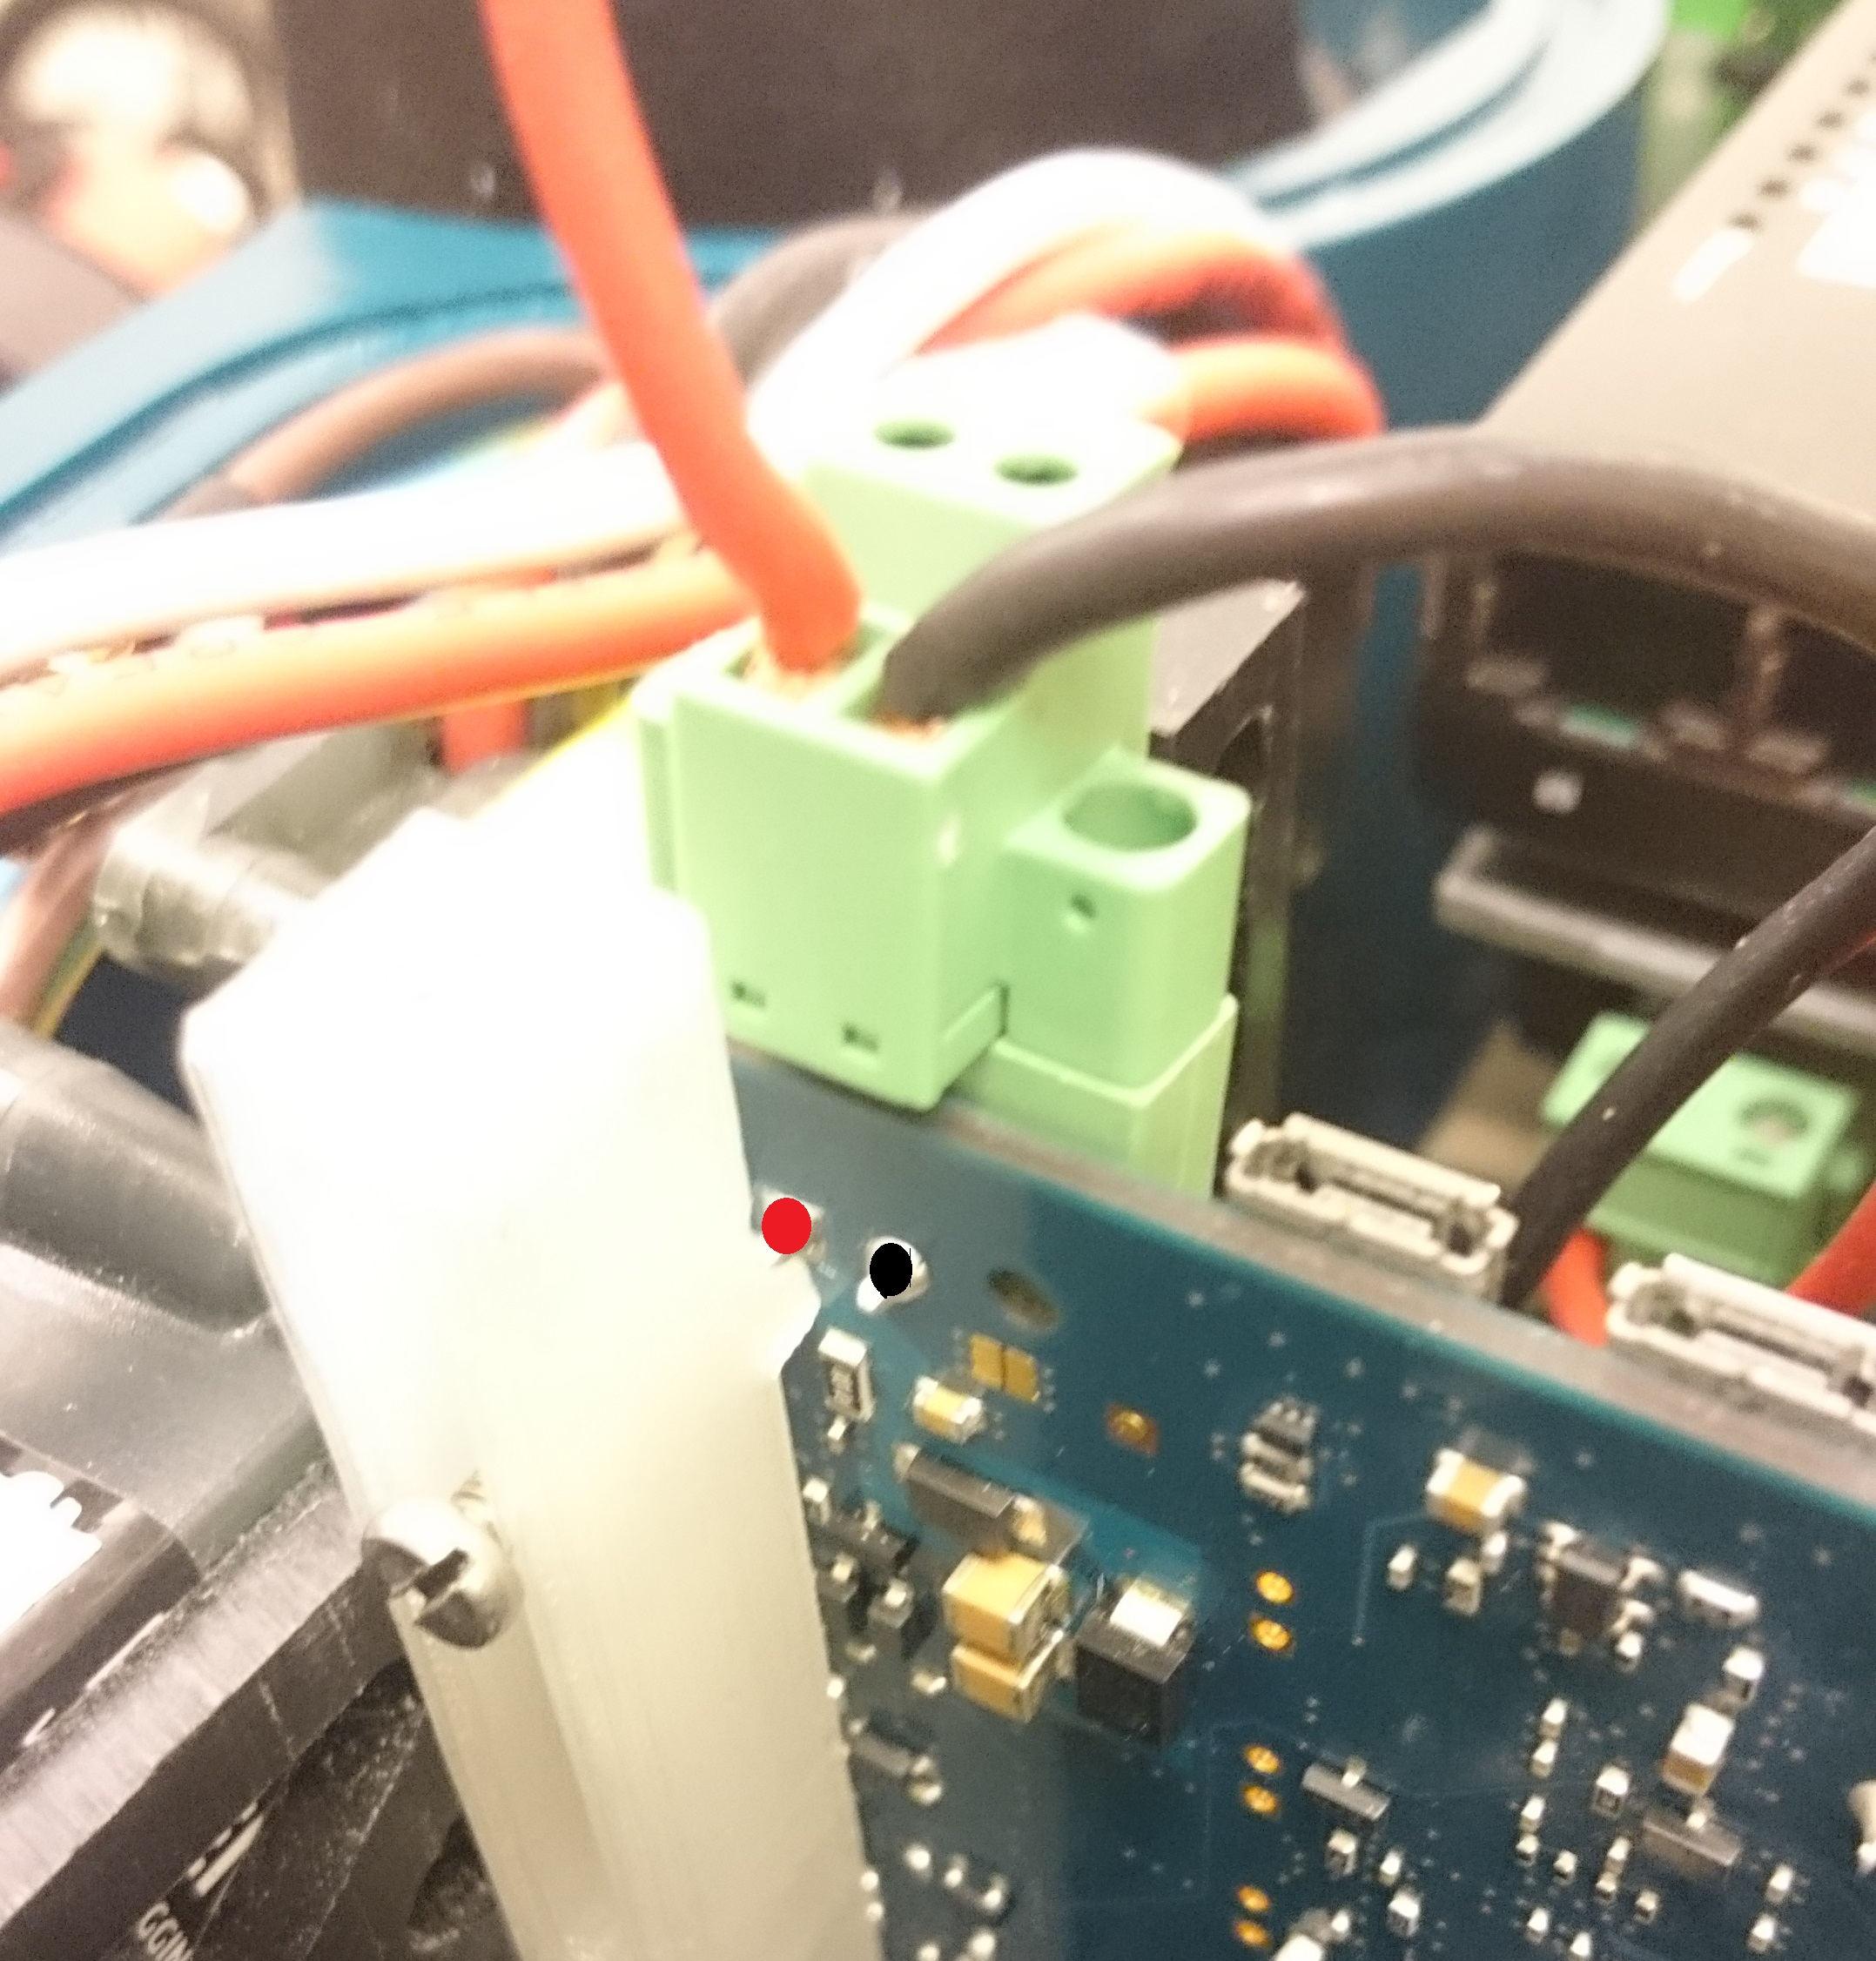
\includegraphics[width=80mm]{Gimme-power.jpg}
		\caption{Measure on the black and red dot, there should be 12 V between them.}
		\label{GimmePower}
	\end{center}
\end{figure}
If there is no power to the GIMME-2 card, make sure to check the connections back to the batteries from the GIMME-2. Make sure to check the cables and the power board for the GIMME-2. Important to remember when checking this power board is that the card is inverted so that the plane is Vcc and that the trace is ground. The input to this board should 24 V and the output 12 V. 

If all of these seem to be correct, the problem is probably with the GIMME-2 board, this is not easy to fix, replace the card. If the card seems to be working but the vision system still is not, the problem might be in the software for the vision system. 

\begin{tabular}{| l | c |}
\hline
Check point & Measured \\ \hline
Measure power input in GIMME-2 & \\ \hline
Check cables & \\ \hline
GIMME-2 power board & \\ \hline
\end{tabular} 

\subsubsection*{Inclusion/Exclusion points}
This test counts as a pass if the problem can be found and the GIMME-2 board starts working. All other results will count as fails. 
\subsubsection*{Special requirements}
There are no parameters for this category. 

\subsection{Markers are not releasing as they are supposed to}
\subsubsection*{Purpouse of the test case}
The markers might not release as they are supposed to, the purpouse of this test is to find out why this problem occurs. 
\subsubsection*{Description}
This test is designed to find the reason to why the markers are not releasing properly. 
\subsubsection*{Resources}
Complete system including electronics and mechanics.  
\subsubsection*{Preconditions}
For this test case to be relevant the markers should not be releasing as they are supposed to. 
\subsubsection*{Post conditions}
The markers release when supposed to. 
\subsubsection*{Flow of events}
The first thing to check is that the markers are free to release. The next thing to check is to make sure that the solenoid is connected properly. Make sure to also check that the actuator shield is connected properly to its CAN card and that the CAN card is connected properly to the stack. After doing all of these things the next thing is to make a complete unit test of the actuator shield, and if that does not work a unit test on the CAN card should be done.

\begin{tabular}{| l | c |}
\hline
Check point & Measured \\ \hline
Marker can release properly &  \\ \hline
Solenoid connection &  \\ \hline
Actuator shield connection &  \\ \hline
CAN connection & \\ \hline
Actuator shield unit test & \\ \hline
CAN card unit test & \\ \hline
\end{tabular} 
\subsubsection*{Inclusion/Exclusion points}
There are no exclusion points to this test. 
\subsubsection*{Special requirements}
There are no special requirements for this test. 

\subsection{A sensor is giving out a faulty value}
\subsubsection*{Purpouse of the test case}
There are a number of sensors on the Naiad system, the purpouse of this test is to identify the problem when one of them is giving out a faulty value. 
\subsubsection*{Description}
It might happen that one of the sensors give out a fault value, which could make the AUV act inappropriately. This test is designed to ensure how to find the problem if that were to happen. 
\subsubsection*{Resources}
Electronics of Naiad including the affected sensor(s).
\subsubsection*{Preconditions}
A sensor in the system is giving out a faulty value when reading it in software. 
\subsubsection*{Post conditions}
The desired post condition is that the sensor works properly. 
\subsubsection*{Flow of events}
The thing to start with is checking that the sensor is connected properly, that the sensor shield it is attached to is mounted on its CAN-card properly and that the CAN-card is properly connected to its stack. If all of this is properly connected and the sensor is still giving out a faulty value, turn to the respective unit test of that sensor or the card it is mounted to. If the problem is still not resolved, make sure to do a complete unit test on the CAN card the sensor is connected to.

\begin{tabular}{| l | c |}
\hline
Check point & Measured \\ \hline
Sensor connection &  \\ \hline
Shield connection &  \\ \hline
CAN connection & \\ \hline
Sensor shield unit test & \\ \hline
CAN card unit test & \\ \hline
\end{tabular}   
\subsubsection*{Inclusion/Exclusion points}
This test does not test the sensors, it is just testing the connections and the mountings. 
\subsubsection*{Special requirements}
No special requirements for this test. 

\subsection{System does not start}
\label{nostart}
\subsubsection*{Purpouse of the test case}
The purpouse of this test is to find out what is wrong if the system will not start when you power it up. 
\subsubsection*{Description}
This test was created to ease problems with a system that does not start as it is supposed to. 
\subsubsection*{Resources}
Complete Naiad with electronics, batteries and hull, a multimeter,
\subsubsection*{Preconditions}
The robot is not starting when the batteries are plugged in. 
\subsubsection*{Post conditions}
For passing this test, the system should start after this test. 
\subsubsection*{Flow of events}
Start by checking the connection from the batteries to the power cords. It they are connected continue with checking the power level on the batteries. This can be done using a multimeter. The batteries should measure above 22 V, if using a battery monitor all cells should be indicating green. If the voltage is running low, try charging the batteries and then start up the system. If the charger will not charge a battery that could mean that a cell is damaged, discard the battery. 

The next step is to check the Power Supply Unit, the first thing to look for is the fuse on the PSU. This is marked in fig. \ref{PSU_fuse}
\begin{figure}[!ht]
	\begin{center}
		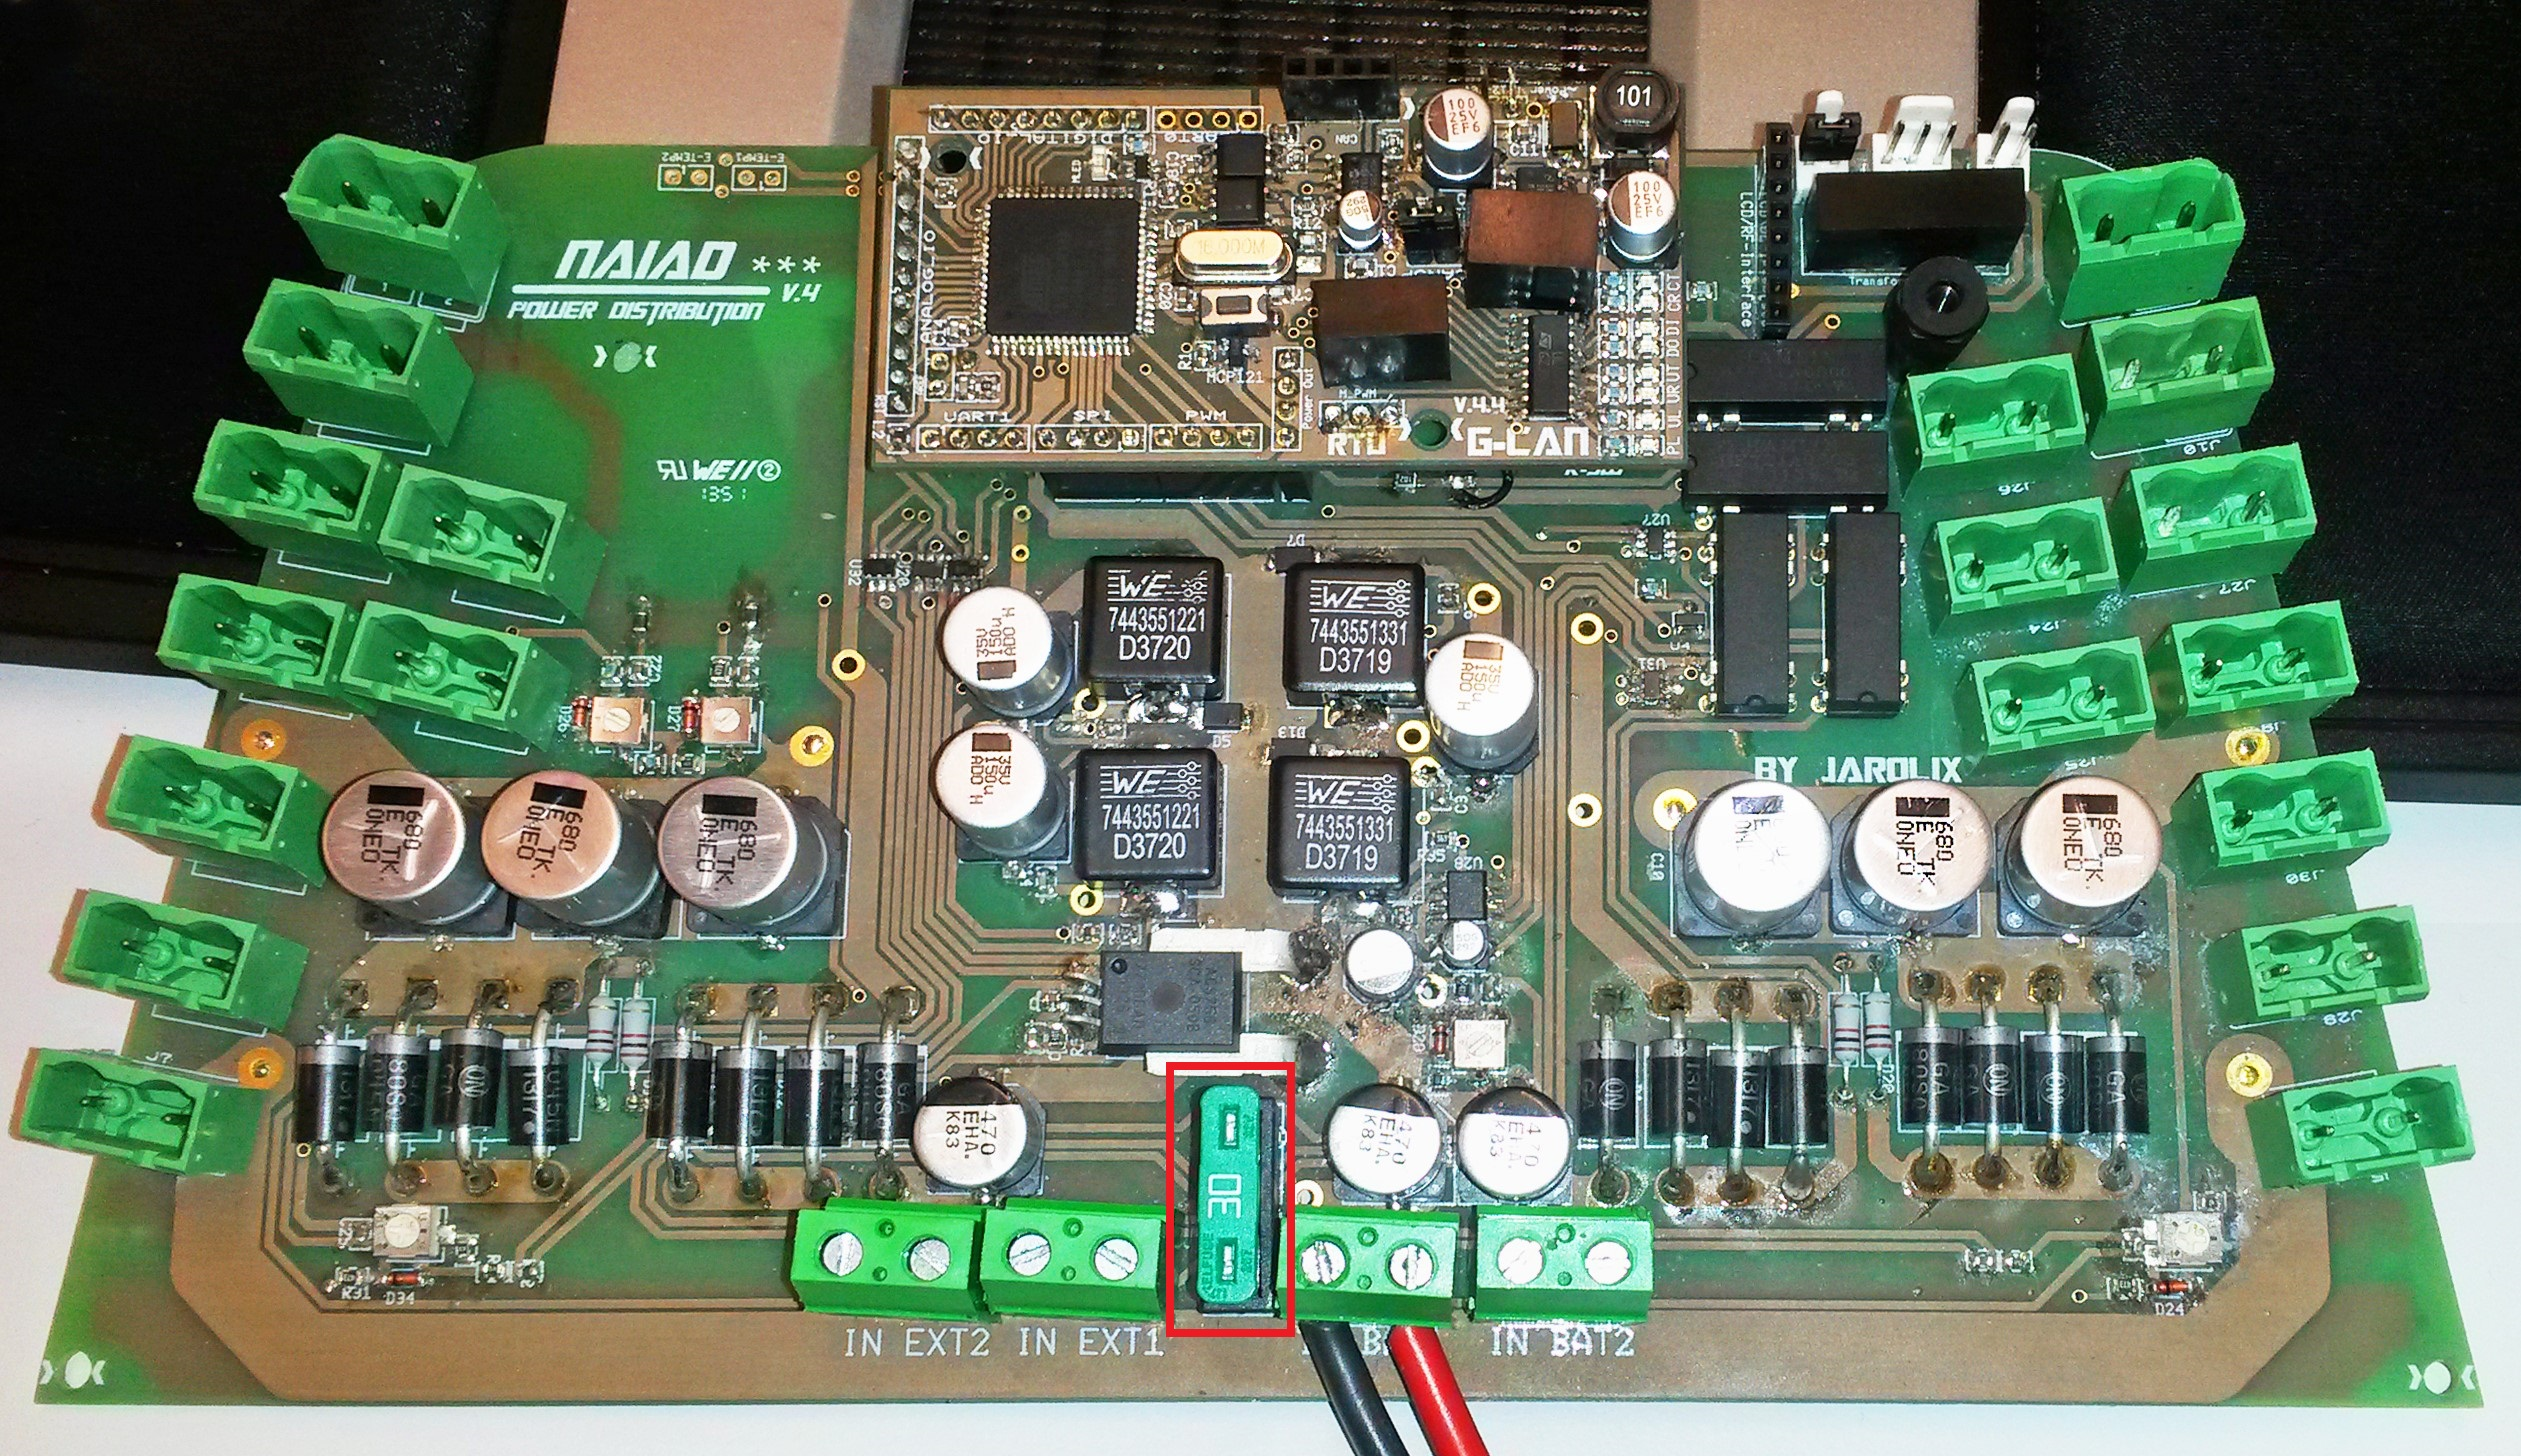
\includegraphics[width=80mm]{powerboard_fuse.jpg}
		\caption{The red square indicates where the fuse can be found on the PSU}
		\label{PSU_fuse}
	\end{center}
\end{figure}
If the fuse is broken, make sure to replace it with a new one. Test if the system will start again. If this did not work, make a complete unit test of the PSU. 

\begin{tabular}{| l | c |}
\hline
Check point & Measured \\ \hline
Battery connection &  \\ \hline
Power level batteries &  \\ \hline
Fuse status & \\ \hline
PSU unit test & \\ \hline
\end{tabular} 
\subsubsection*{Inclusion/Exclusion points}
AVVAKTAR!
\subsubsection*{Special requirements}
There are no special requirements for this test. 

\subsection{Is the hull water tight}
\subsubsection*{Purpouse of the test case}
The purpouse of this test is to make sure that the hull is waterproof and that it will not leak when put in water. 
\subsubsection*{Description}
Testing if the hull is watertight is a continuation from the unit test of the hull. This test can be found at \ref{Hulltest}.
\subsubsection*{Resources}
Required resources for this test is the hull of Naiad, some paper, petroleum jelly, a long rope, and weights (for example in a weight belt for diving). A pool to sink the hull in is also required. 
\subsubsection*{Preconditions}
The preconditions for this test is to fill the inside of the hull with toiletpaper to easier see if there is any intake of water. The hull should then be closed according to the specification found in \ref{Hulltest}.
\subsubsection*{Post conditions}
The post conditions are the same as the preconditions. 
\subsubsection*{Flow of events}
Enough weights to sink the hull should be attached to the hull, make sure that the weights can not fall of when the hull moves around. It should be sunk to the bottom of the water and then left there for at least five minutes. Then it could be lifted from the water and dried on the outside. The lid should then be opened and the inside examined to see that there is no water on the inside. 

\begin{tabular}{| l | c |}
\hline
Check point & Measured \\ \hline
Closed properly &  \\ \hline
Weights attatched &  \\ \hline
Sunk & \\ \hline
Lifted & \\ \hline
Outside dried & \\ \hline
Inside dry & \\ \hline
\end{tabular}
\subsubsection*{Inclusion/Exclusion points}
The depth to which the hull is waterproof is not tested in this test. 
\subsubsection*{Special requirements}
There are no special requirements for this test. 

\subsection{Motor not starting}
This case is a common problem in which one or more motor(s) for some reason is not starting.
\subsubsection*{Purpouse of the test}
The purpose of this test is to identify the problem with the motor and find out why the motor is not running. 
\subsubsection*{Description}
The test is designed to identify any problems with why a motor is not running. 
\subsubsection*{Resources}
One person is required to perform the test. 
\subsubsection*{Preconditions}
The motor is not running on command.
\subsubsection*{Post conditions}
The desired post condition of this test is a motor that is running. 
\subsubsection*{Flow of events}
When the motor is not working that means one of two things. Either the motor is completely quiet or the motor gives out a 2Hz beep-signal. 

If the motor(s) is completely quiet that would imply that there is no power to the motor. In that case all the cables to the power supply needs to be checked. These cables are thick, one is red and the other one is black, and will come from the motor controller and should be plugged in to the power supply unit. Also the cables to the motors need checking, that is three cables, they are red, white and black from the motor controller and should match the shrink tubing on the cables going out to the motors. When checking the cables - make sure that the conwtb-female has not started to be loose, in this case the contact needs to be switched to a new one. 

If the motor(s) are giving out a beeping signal at 2Hz, that would mean that there is no signal to the motor(s). In this case the signal cable need checking. This cable is orange/red/black and run from the motor controller to the motor extension board. Make sure that the motor extension board is properly connected to the CAN-card. Also make sure that the CAN-card is properly connected to the stack.  

If all the cables and cards are plugged in as they are supposed and the system is still quiet this could mean that there is no power in the system, in this case, nothing should be working and all LEDs should be turned off. In this case, check that the batteries are plugged in and that they are charged properly. How to do this is better specified under \ref{nostart}.

If there is power in the system even if the motor is silent and all the cables are connected correctly then this would mean that the power supply unit is not working properly. To test this card, use test \ref{subsec:psu}.

\begin{tabular}{| l | c |}
\hline
Check point & Measured \\ \hline
2Hz beeps &  \\ \hline
Power cables to motor controller &  \\ \hline
Cables from motor controller & \\ \hline
conwtb-female & \\ \hline
Signal cable to motor controller & \\ \hline
Motor extension board & \\ \hline
CAN-card connection & \\ \hline
System power & \\ \hline
PSU unit test & \\ \hline
\end{tabular}
\subsubsection*{Inclusion/Exclusion points}
This test does not test wether the motor is working or not. If the test is failed one could further test this.  
\subsubsection*{Special requirements}
There are no special requirements. 

\end{document}